% !TEX TS-program = knitr
\documentclass{article}\usepackage{graphicx, color}
%% maxwidth is the original width if it is less than linewidth
%% otherwise use linewidth (to make sure the graphics do not exceed the margin)
\makeatletter
\def\maxwidth{ %
  \ifdim\Gin@nat@width>\linewidth
    \linewidth
  \else
    \Gin@nat@width
  \fi
}
\makeatother

\IfFileExists{upquote.sty}{\usepackage{upquote}}{}
\definecolor{fgcolor}{rgb}{0.2, 0.2, 0.2}
\newcommand{\hlnumber}[1]{\textcolor[rgb]{0,0,0}{#1}}%
\newcommand{\hlfunctioncall}[1]{\textcolor[rgb]{0.501960784313725,0,0.329411764705882}{\textbf{#1}}}%
\newcommand{\hlstring}[1]{\textcolor[rgb]{0.6,0.6,1}{#1}}%
\newcommand{\hlkeyword}[1]{\textcolor[rgb]{0,0,0}{\textbf{#1}}}%
\newcommand{\hlargument}[1]{\textcolor[rgb]{0.690196078431373,0.250980392156863,0.0196078431372549}{#1}}%
\newcommand{\hlcomment}[1]{\textcolor[rgb]{0.180392156862745,0.6,0.341176470588235}{#1}}%
\newcommand{\hlroxygencomment}[1]{\textcolor[rgb]{0.43921568627451,0.47843137254902,0.701960784313725}{#1}}%
\newcommand{\hlformalargs}[1]{\textcolor[rgb]{0.690196078431373,0.250980392156863,0.0196078431372549}{#1}}%
\newcommand{\hleqformalargs}[1]{\textcolor[rgb]{0.690196078431373,0.250980392156863,0.0196078431372549}{#1}}%
\newcommand{\hlassignement}[1]{\textcolor[rgb]{0,0,0}{\textbf{#1}}}%
\newcommand{\hlpackage}[1]{\textcolor[rgb]{0.588235294117647,0.709803921568627,0.145098039215686}{#1}}%
\newcommand{\hlslot}[1]{\textit{#1}}%
\newcommand{\hlsymbol}[1]{\textcolor[rgb]{0,0,0}{#1}}%
\newcommand{\hlprompt}[1]{\textcolor[rgb]{0.2,0.2,0.2}{#1}}%

\usepackage{framed}
\makeatletter
\newenvironment{kframe}{%
 \def\at@end@of@kframe{}%
 \ifinner\ifhmode%
  \def\at@end@of@kframe{\end{minipage}}%
  \begin{minipage}{\columnwidth}%
 \fi\fi%
 \def\FrameCommand##1{\hskip\@totalleftmargin \hskip-\fboxsep
 \colorbox{shadecolor}{##1}\hskip-\fboxsep
     % There is no \\@totalrightmargin, so:
     \hskip-\linewidth \hskip-\@totalleftmargin \hskip\columnwidth}%
 \MakeFramed {\advance\hsize-\width
   \@totalleftmargin\z@ \linewidth\hsize
   \@setminipage}}%
 {\par\unskip\endMakeFramed%
 \at@end@of@kframe}
\makeatother

\definecolor{shadecolor}{rgb}{.97, .97, .97}
\definecolor{messagecolor}{rgb}{0, 0, 0}
\definecolor{warningcolor}{rgb}{1, 0, 1}
\definecolor{errorcolor}{rgb}{1, 0, 0}
\newenvironment{knitrout}{}{} % an empty environment to be redefined in TeX

\usepackage{alltt}

\usepackage{amsfonts}
\usepackage{amsmath}
\usepackage{amssymb}
\usepackage{amsthm}
\usepackage{caption}
\usepackage{color}
\usepackage{enumerate}
\usepackage{fancyhdr}
\usepackage{hyperref}
\usepackage{graphicx}
\usepackage{latexsym}
\usepackage{listings}
\usepackage{mathrsfs}
\usepackage{natbib}
\usepackage[nottoc]{tocbibind}
\usepackage{url}

\providecommand{\all}{\ \forall \ }
\providecommand{\bs}{\backslash}
\providecommand{\e}{\varepsilon}
\providecommand{\E}{\ \exists \ }
\providecommand{\lm}[2]{\lim_{#1 \rightarrow #2}}
\providecommand{\m}[1]{\mathbb{#1}}
\providecommand{\nv}{{}^{-1}}
\providecommand{\ov}[1]{\overline{#1}}
\providecommand{\p}{\newpage}
\providecommand{\q}{$\quad$ \newline}
\providecommand{\rt}{\rightarrow}
\providecommand{\Rt}{\Rightarrow}
\providecommand{\vc}[1]{\boldsymbol{#1}}
\providecommand{\wh}[1]{\widehat{#1}}

%\renewcommand\bibname{References}
%\renewcommand{\thesection}{Problem \arabic{section}}
%\renewcommand{\thesubsection}{Part \alph{subsection}}
\numberwithin{equation}{section}

\fancyhead{}
\fancyfoot{}
\fancyhead[R]{\thepage}
\fancyhead[C]{Landau}

\hypersetup{
    colorlinks,
    citecolor=black,
    filecolor=black,
    linkcolor=black,
    urlcolor=blue
}

\definecolor{dkgreen}{rgb}{0,0.6,0}
\definecolor{gray}{rgb}{0.5,0.5,0.5}
\definecolor{mauve}{rgb}{0.58,0,0.82}

\lstset{ 
  language=C,                % the language of the code
  basicstyle=\Large,           % the size of the fonts that are used for the code
  numberstyle= \tiny \color{white},  % the style that is used for the line-numbers
  stepnumber=2,                   % the step between two line-numbers. 
  numbersep=5pt,                  % how far the line-numbers are from the code
  backgroundcolor=\color{white},      % choose the background color. You must add \usepackage{color}
  showspaces=false,               % show spaces adding particular underscores
  showstringspaces=false,         % underline spaces within strings
  showtabs=false,                 % show tabs within strings adding particular underscores
  frame=lrb,                   % adds a frame around the code
  rulecolor=\color{black},        % if not set, the frame-color may be changed on line-breaks within not-black text 
  tabsize=2,                      % sets default tabsize to 2 spaces
  captionpos=t,                   % sets the caption-position 
  breaklines=true,                % sets automatic line breaking
  breakatwhitespace=false,        % sets if automatic breaks should only happen at whitespace
  title=\lstname,                   % show the filename of files included with \lstinputlisting;
  keywordstyle=\color{blue},          % keyword style
  commentstyle=\color{gray},       % comment style
  stringstyle=\color{dkgreen},         % string literal style
  escapeinside={\%*}{*)},            % if you want to add LaTeX within your code
  morekeywords={*, ...},               % if you want to add more keywords to the set
  xleftmargin=0.053in, % left horizontal offset of caption box
  xrightmargin=-.03in % right horizontal offset of caption box
}

\DeclareCaptionFont{white}{\color{white}}
\DeclareCaptionFormat{listing}{\parbox{\textwidth}{\colorbox{gray}{\parbox{\textwidth}{#1#2#3}}\vskip-0.05in}}
\captionsetup[lstlisting]{format = listing, labelfont = white, textfont = white}
% For caption-free listings, comment out the 3 lines above and uncomment the 2 lines below.
% \captionsetup{labelformat = empty, labelsep = none}
% \lstset{frame = single}






\begin{document}



\begin{flushleft}


\begin{center} \LARGE
STAT 305 D Homework 4 
\end{center}
\begin{center} \Large
Due February 21, 2012 at 12:40 PM in class
\end{center}


\begin{enumerate}[1. ]

\item Vardeman and Jobe chapter 4 section 2 problem 1 (page 161). The data are available at \url{http://will-landau.com/data/csv/polypolyols.csv}. 

\setkeys{Gin}{width=.75\textwidth} 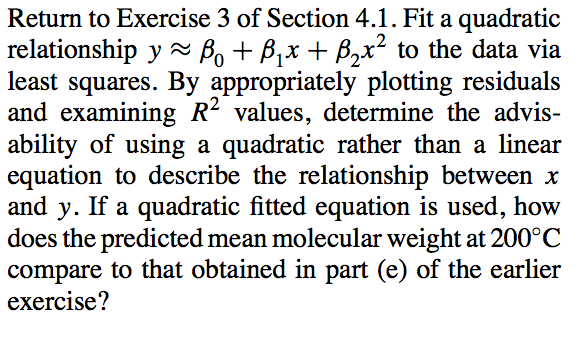
\includegraphics{../../fig/ch4s2p1.png}

The relevant information from section 4.1 exercise 3 is this: The article �Polyglycol Modified Poly (Ethylene Ether Carbonate) Polyols by Molecular Weight Advancement� by R. Harris (Journal of Applied Poly- mer Science, 1990) contains some data on the effect of reaction temperature on the molecular weight of resulting poly polyols. The data for eight experimental runs at temperatures 165${}^\circ$C and above are as follows. Here, $x$ is pot temperature (${}^\circ$) and $y$ is average molecular weight.


% latex table generated in R 2.15.1 by xtable 1.7-0 package
% Sun Feb 17 21:31:48 2013
\begin{table}[ht]
\begin{center}
\begin{tabular}{rr}
 x & y \\ 
  \hline
165.00 & 808.00 \\ 
  176.00 & 940.00 \\ 
  188.00 & 1183.00 \\ 
  205.00 & 1545.00 \\ 
  220.00 & 2012.00 \\ 
  235.00 & 2362.00 \\ 
  250.00 & 2742.00 \\ 
  260.00 & 2935.00 \\ 
  \end{tabular}
\end{center}
\end{table}






\setkeys{Gin}{width=1\textwidth} 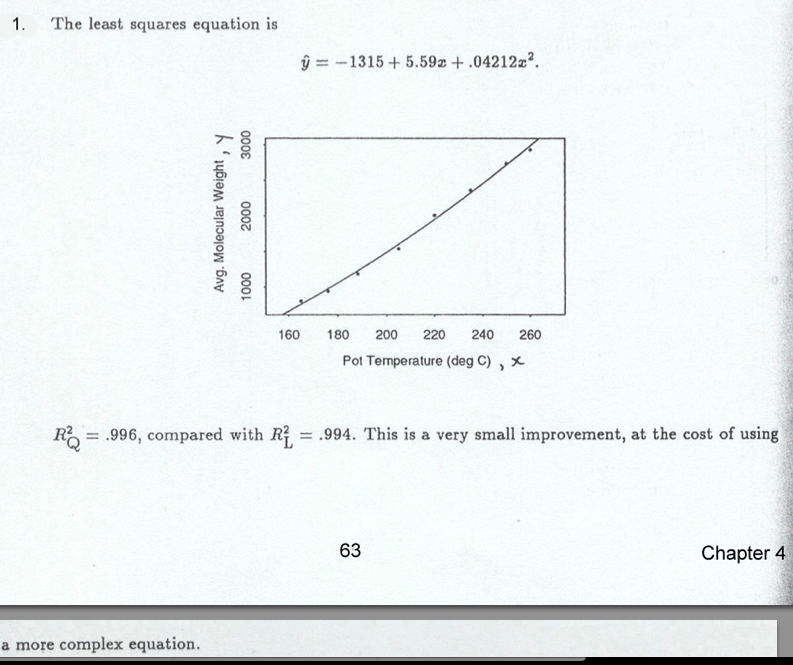
\includegraphics{../../fig/ch4s2p1sol1.png}
\setkeys{Gin}{width=1\textwidth} 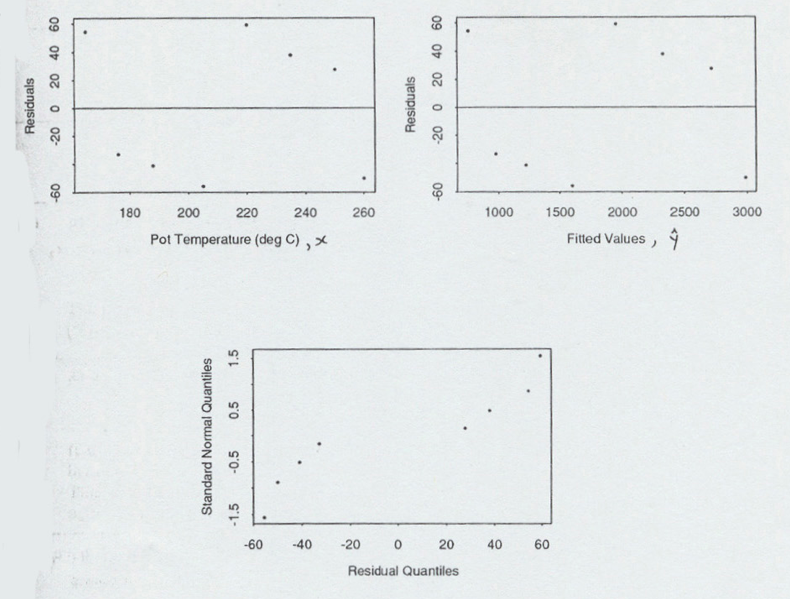
\includegraphics{../../fig/ch4s2p1sol2.png}
\setkeys{Gin}{width=1\textwidth} 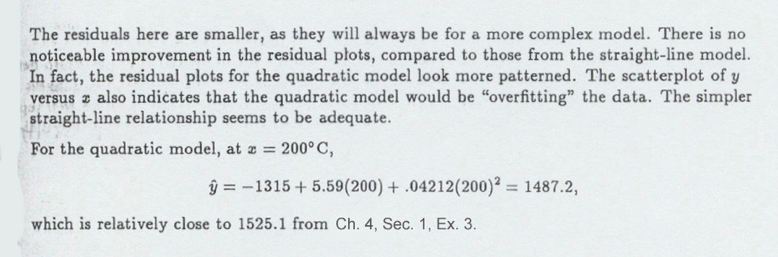
\includegraphics{../../fig/ch4s2p1sol3.png}


\item Vardeman and Jobe chapter 4 section 2 problem 2 parts a-c (page 161). The data are available at \url{http://will-landau.com/stat305/data/csv/pulp.csv}. Here are some data taken from the article �Chemithermomechanical Pulp from Mixed High Density Hardwoods� by Miller, Shankar, and Peterson (Tappi Journal, 1988). Given are the percent NaOH used as a pretreatment chemical, x1, the pretreatment time in minutes, x2, and the resulting value of a specific surface area variable, y (with units of cm3/g), for nine batches of pulp produced from a mixture of hardwoods at a treatment temperature of 75${}^\circ$ C in mechanical pulping.




\setkeys{Gin}{width=.75\textwidth} 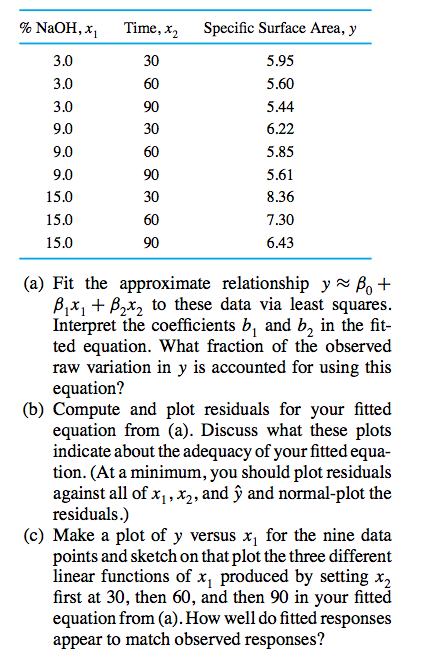
\includegraphics{../../fig/ch4s2p2.png}

\setkeys{Gin}{width=1\textwidth} 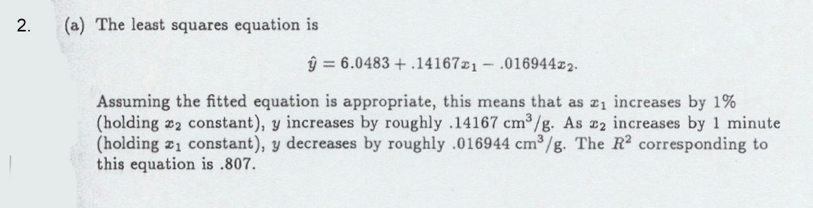
\includegraphics{../../fig/ch4s2p2asol.png}
\setkeys{Gin}{width=1\textwidth} 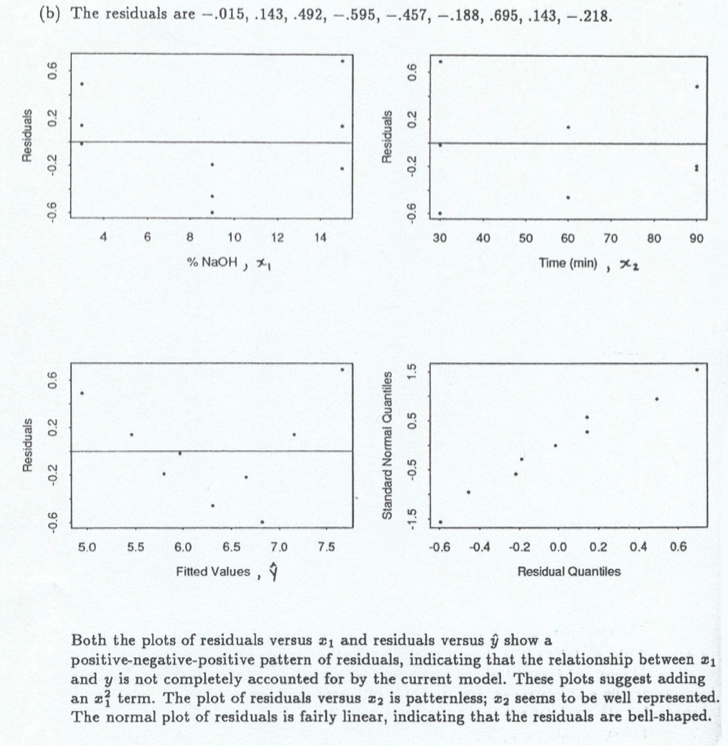
\includegraphics{../../fig/ch4s2p2bsol.png}
\setkeys{Gin}{width=1\textwidth} 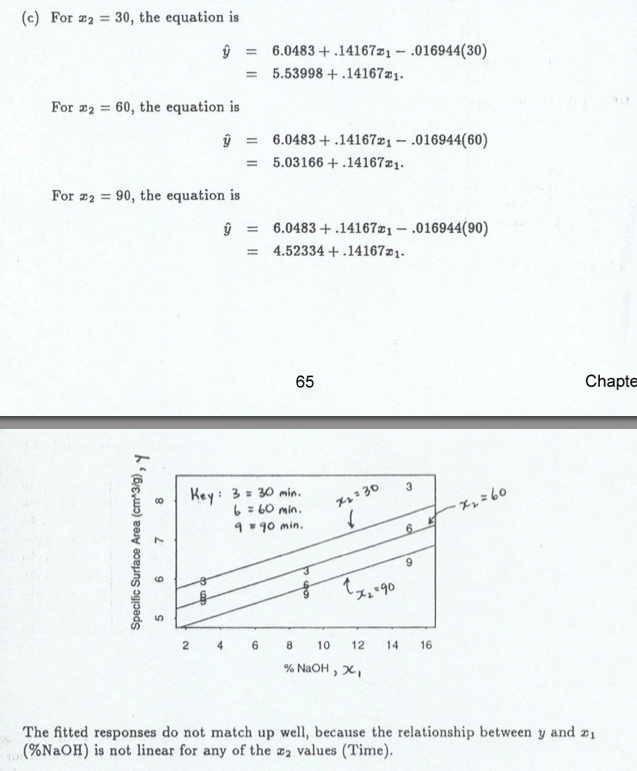
\includegraphics{../../fig/ch4s2p2csol.png}











\clearpage
\item 

\setkeys{Gin}{width=1\textwidth} 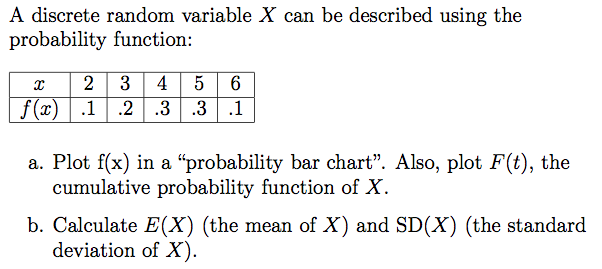
\includegraphics{../../fig/h5p1.png}
\setkeys{Gin}{width=1\textwidth} 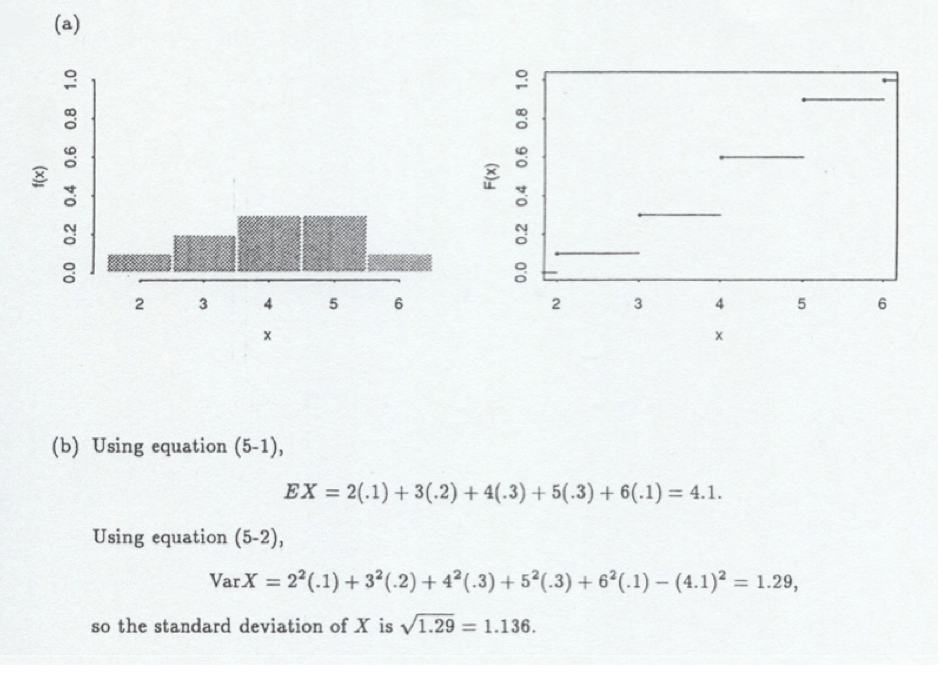
\includegraphics{../../fig/h5p1sol.png}
\clearpage
\item

\setkeys{Gin}{width=1\textwidth} 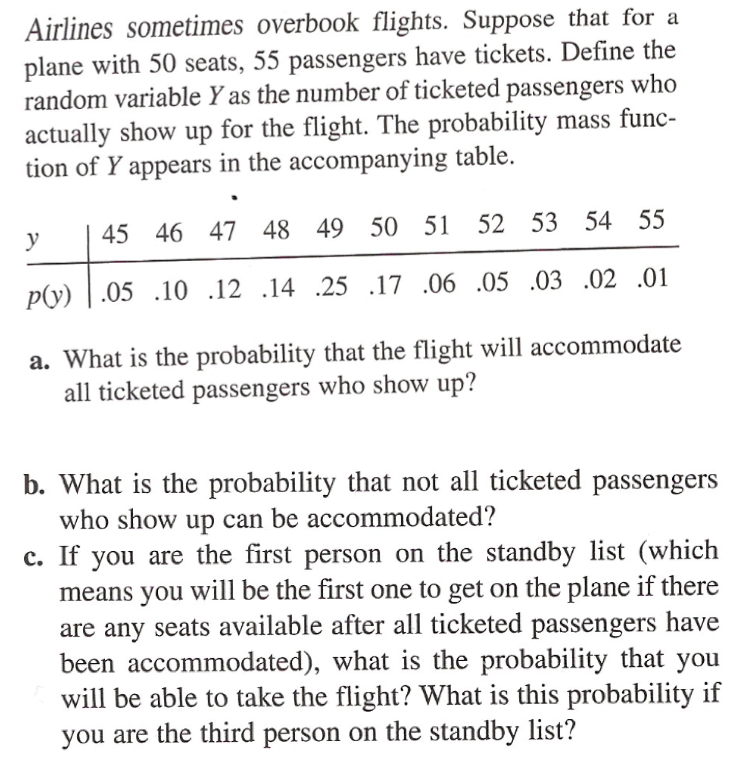
\includegraphics{../../fig/h5p2.png}
\setkeys{Gin}{width=1\textwidth} 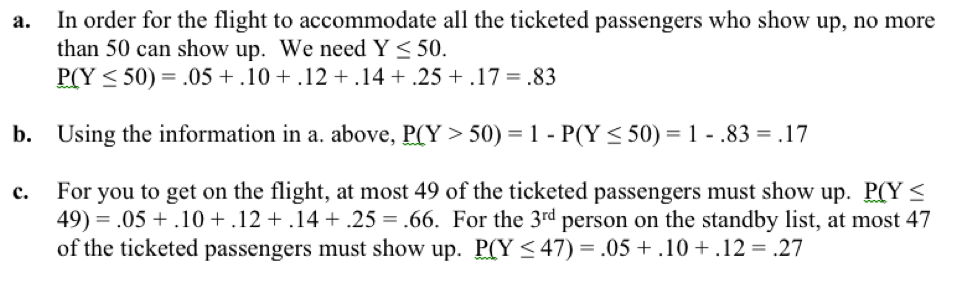
\includegraphics{../../fig/h5p2sol.png}
\clearpage
\item

\setkeys{Gin}{width=1\textwidth} 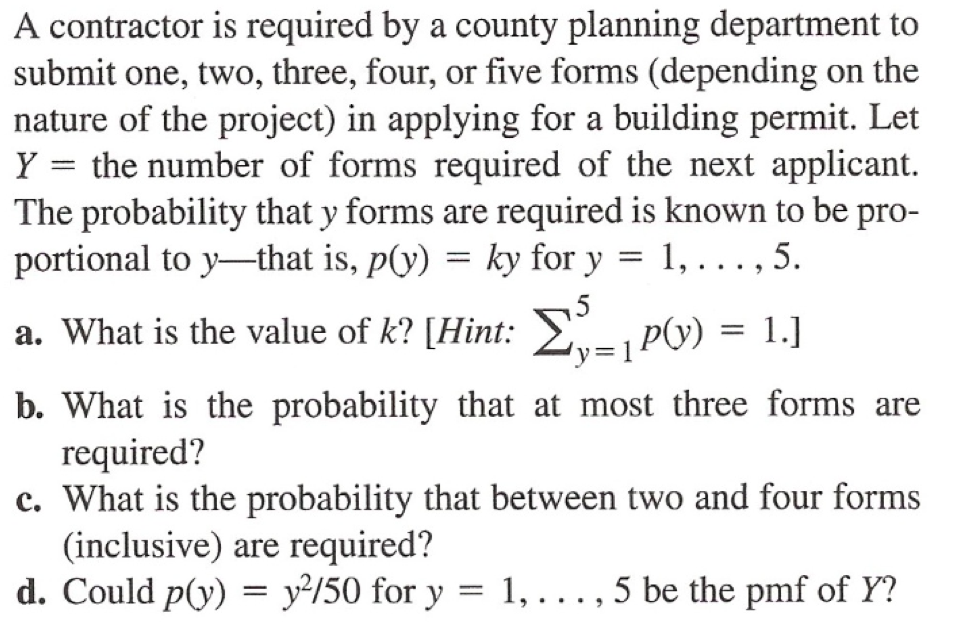
\includegraphics{../../fig/h5p3.png}
\setkeys{Gin}{width=1\textwidth} 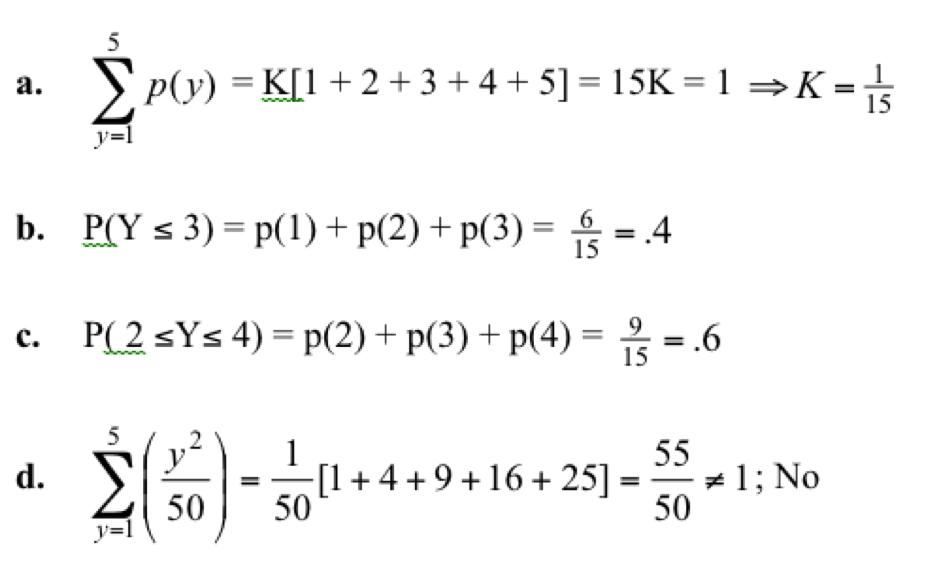
\includegraphics{../../fig/h5p3sol.png}
























\item Weekly feedback. You get full credit as long as you write something.
\begin{enumerate}[1. ]
\item Is there any aspect of the subject matter that you currently struggle with? If so, what specifically do you find difficult or confusing? The more detailed you are, the better I can help you.

{\color{red} You got full credit as long as you wrote something.}
\item Do you have any questions or concerns about the material, class logistics, or anything else? If so, fire away.
{\color{red} You got full credit as long as you wrote something.}
\end{enumerate}
\end{enumerate}




\end{flushleft}
%\newpage 
%\nocite{*}
%\bibliographystyle{plainnat} 
%\bibliography{}
\end{document}
